% Mo Jabeen Template for docs 

\documentclass[11pt]{scrartcl} % Font size

%%%%%%%%%%%%%%%%%%%%%%%%%%%%%%%%%%%%%%%%%
% Wenneker Assignment
% Structure Specification File
% Version 2.0 (12/1/2019)
%
% This template originates from:
% http://www.LaTeXTemplates.com
%
% Authors:
% Vel (vel@LaTeXTemplates.com)
% Frits Wenneker
%
% License:
% CC BY-NC-SA 3.0 (http://creativecommons.org/licenses/by-nc-sa/3.0/)
% 
%%%%%%%%%%%%%%%%%%%%%%%%%%%%%%%%%%%%%%%%%

%----------------------------------------------------------------------------------------
%	PACKAGES AND OTHER DOCUMENT CONFIGURATIONS
%----------------------------------------------------------------------------------------

\usepackage{amsmath, amsfonts, amsthm} % Math packages

\usepackage{listings} % Code listings, with syntax highlighting

\usepackage[english]{babel} % English language hyphenation

\usepackage{graphicx} % Required for inserting images
\graphicspath{{Figures/}{./}} % Specifies where to look for included images (trailing slash required)

\usepackage{booktabs} % Required for better horizontal rules in tables

\numberwithin{equation}{section} % Number equations within sections (i.e. 1.1, 1.2, 2.1, 2.2 instead of 1, 2, 3, 4)
\numberwithin{figure}{section} % Number figures within sections (i.e. 1.1, 1.2, 2.1, 2.2 instead of 1, 2, 3, 4)
\numberwithin{table}{section} % Number tables within sections (i.e. 1.1, 1.2, 2.1, 2.2 instead of 1, 2, 3, 4)

\setlength\parindent{0pt} % Removes all indentation from paragraphs

\usepackage{enumitem} % Required for list customisation
\setlist{noitemsep} % No spacing between list items

\usepackage{array}
\newcolumntype{P}[1]{>{\centering\arraybackslash}p{#1}} %Allows centering of tables

\usepackage[
backend=biber,
style=ieee,
sorting=ynt
]{biblatex}

\addbibresource{refs.bib} %Imports bibliography file

%----------------------------------------------------------------------------------------
%	DOCUMENT MARGINS
%----------------------------------------------------------------------------------------

\usepackage{geometry} % Required for adjusting page dimensions and margins

\geometry{
	paper=a4paper, % Paper size, change to letterpaper for US letter size
	top=2.5cm, % Top margin
	bottom=3cm, % Bottom margin
	left=3cm, % Left margin
	right=3cm, % Right margin
	headheight=0.75cm, % Header height
	footskip=1.5cm, % Space from the bottom margin to the baseline of the footer
	headsep=0.75cm, % Space from the top margin to the baseline of the header
	%showframe, % Uncomment to show how the type block is set on the page
}

%----------------------------------------------------------------------------------------
%	FONTS
%----------------------------------------------------------------------------------------

\usepackage[utf8]{inputenc} % Required for inputting international characters
\usepackage[T1]{fontenc} % Use 8-bit encoding

\usepackage{fourier} % Use the Adobe Utopia font for the document

%----------------------------------------------------------------------------------------
%	HEADERS AND FOOTERS
%----------------------------------------------------------------------------------------

\usepackage{scrlayer-scrpage} % Required for customising headers and footers

\ohead*{} % Right header
\ihead*{} % Left header
\chead*{} % Centre header

\ofoot*{} % Right footer
\ifoot*{} % Left footer
\cfoot*{\pagemark} % Centre footer

%----------------------------------------------------------------------------------------
%	SECTION TITLES
%----------------------------------------------------------------------------------------
 % Include the file specifying the document structure and custom commands

%----------------------------------------------------------------------------------------
%	TITLE SECTION
%----------------------------------------------------------------------------------------


\title{	
	\normalfont\normalsize
	\vspace{20pt} % Whitespace
	{\huge Design Patterns}\\ % The meh
	\vspace{12pt} % Whitespace
	\rule{\linewidth}{2pt}\\ % Thick bottom horizontal rule
}

\author{\small Dainish Jabeen} % Your name

\date{\normalsize\today} % Today's date (\today) or a custom date

\begin{document}

\maketitle % Print the title

\section{Introduction}

Patterns describe evolved methods through trail and error, of commonly occurring problems.

\section{SOLID}

\subsubsection{Single Responsibility Principle}

A class should have just one reason to change.

\subsubsection{Open/Close Principle}

Classes should be open for extension but closed for modification.

\subsubsection{Liskov Substitution Principle}

Extending a class, should be able to use objects of the subclass instead of the parent class.

\subsubsection{Interface Segregation Principle}

Clients shouldn't be forced to depend on methods they dont use.

\subsubsection{Dependancy Inversion Principle}

High level classes should not depend on low level classes. Details should depend on abstractions.

\section{Composition}

Preferred to inheritance, the concept is to use interfaces to expand behaviours easily 
(in a plugin method).

\section{Types of patterns}

\textbf{Creational Patterns:} Increase flexibility and reusability.\\

\textbf{Structural Patterns:} Assemble classes to large structures while keeping them flexible and
efficient.\\

\textbf{Behavioural Patterns:} Effective communication and responsibility between modules.

\section{Creational Patterns}

\subsection{Factory}

Create objects in superclass, alter in subclass.\\

The creation of objects is done using the factory method, that changes the 
object returned based on context (normally conditional statements) which is the subclass of a 'Creator' class
. The return type of the function is an abstract so the client receiving 
does not know the details of the object.\\

This abstract type is an interface, which is detailed in concrete implementations that specify
which object is created. Which are directly called via a subclass of the creator. \\

This eases the creation of new objects to be used, and is useful if it is context dependant which
object should be created and used. \\

Can also create a pool of objects, which the factory method checks before creating a new object.\\

\begin{figure}[h] % [h] forces the figure to be output where it is defined in the code (it suppresses floating)
	\centering
	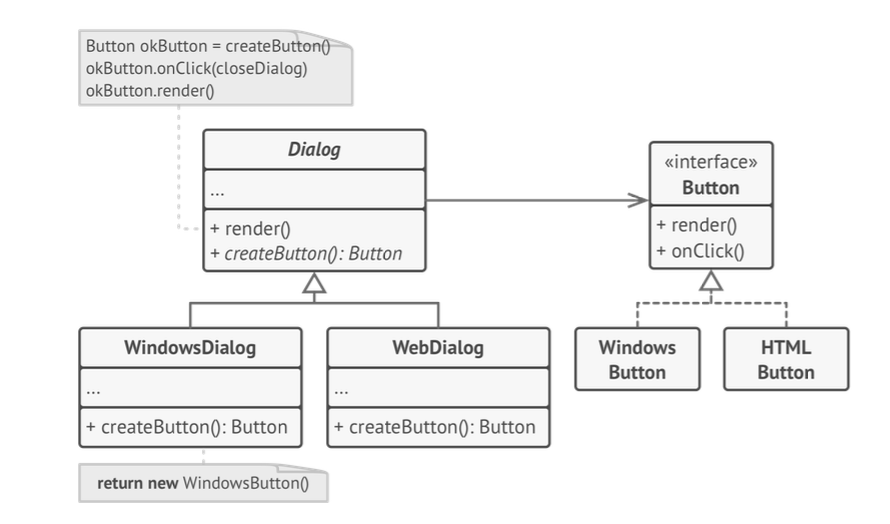
\includegraphics[width=\columnwidth]{Factory.png} % Example image
	\caption{Factory Structure}
	\label{Factory Structure}
\end{figure}

Diagram of structure Figure:\ref{Factory Structure} on Page:\pageref{Factory Structure}.

\subsection{Abstract Factory}

Create families of objects without specifying its implementation.\\

If there matrix of implementations ie feature 1 x feature 2 (furniture x style). An interface is created for each
characteristic on one dimension (interface for each furniture type) and an implementation of each the 
second dimensions characteristic on each interface (implementation for each style type).\\

The abstract factory is the creator interface with an implementation of each of the second dimensions characteristics
(style types) that create each of first dimensions object with that chosen second dim. The return type is an interface of 
the first dimension allowing to use any first dim methods without the client knowing the second dim.
Allowing easy additions of either dims. Extension method for first dimension and plugin method for second dim.\\

\begin{figure}[h] % [h] forces the figure to be output where it is defined in the code (it suppresses floating)
	\centering
	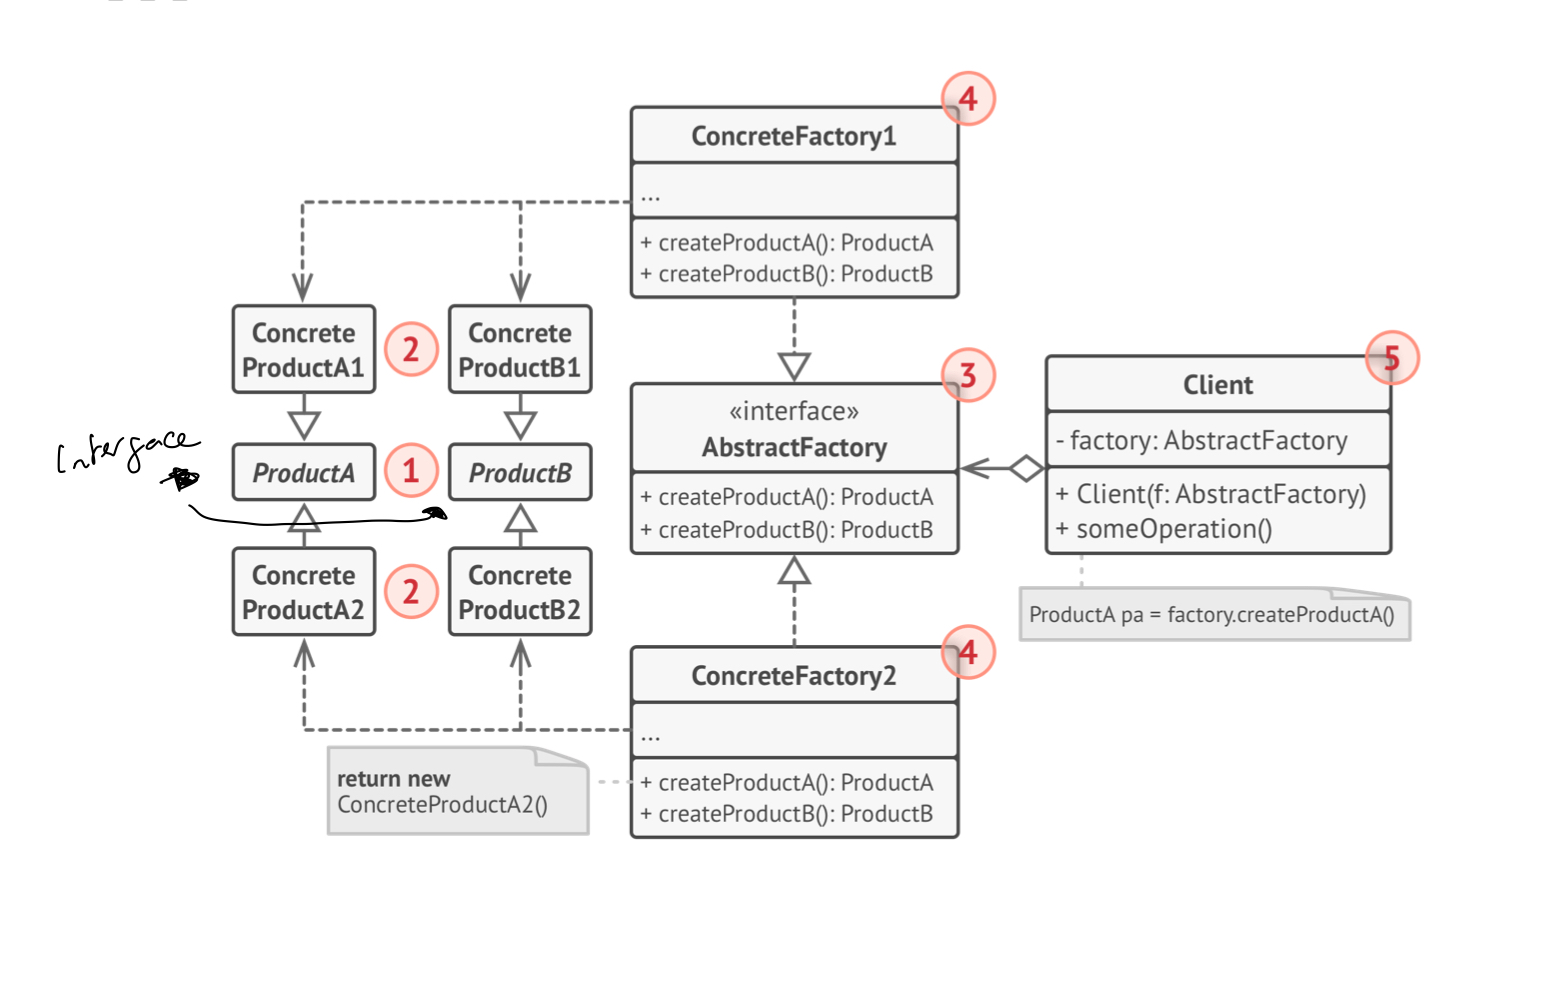
\includegraphics[width=\columnwidth]{Abstract Factory.jpeg} % Example image
	\caption{Abstract Factory Structure}
	\label{Abstract Factory Structure}
\end{figure}

Diagram of structure Figure:\ref{Abstract Factory Structure} on Page:\pageref{Abstract Factory Structure}.

\subsection{Builder}

Using the same construction code to build complex objects.\\

Solving the issues of classes with many parameters, create a builder modules thare implementations of
an interface for the variations in the object. In each builder the parameters will be set,
 you dont need to use all parameters.\\

For easier construction reuse a director module with coded methods of using the builders. The 
client code will use the director via a concrete builder to get the object.\\

This gives you an easy way to extend variations of an object.\\

\begin{figure}[h] % [h] forces the figure to be output where it is defined in the code (it suppresses floating)
	\centering
	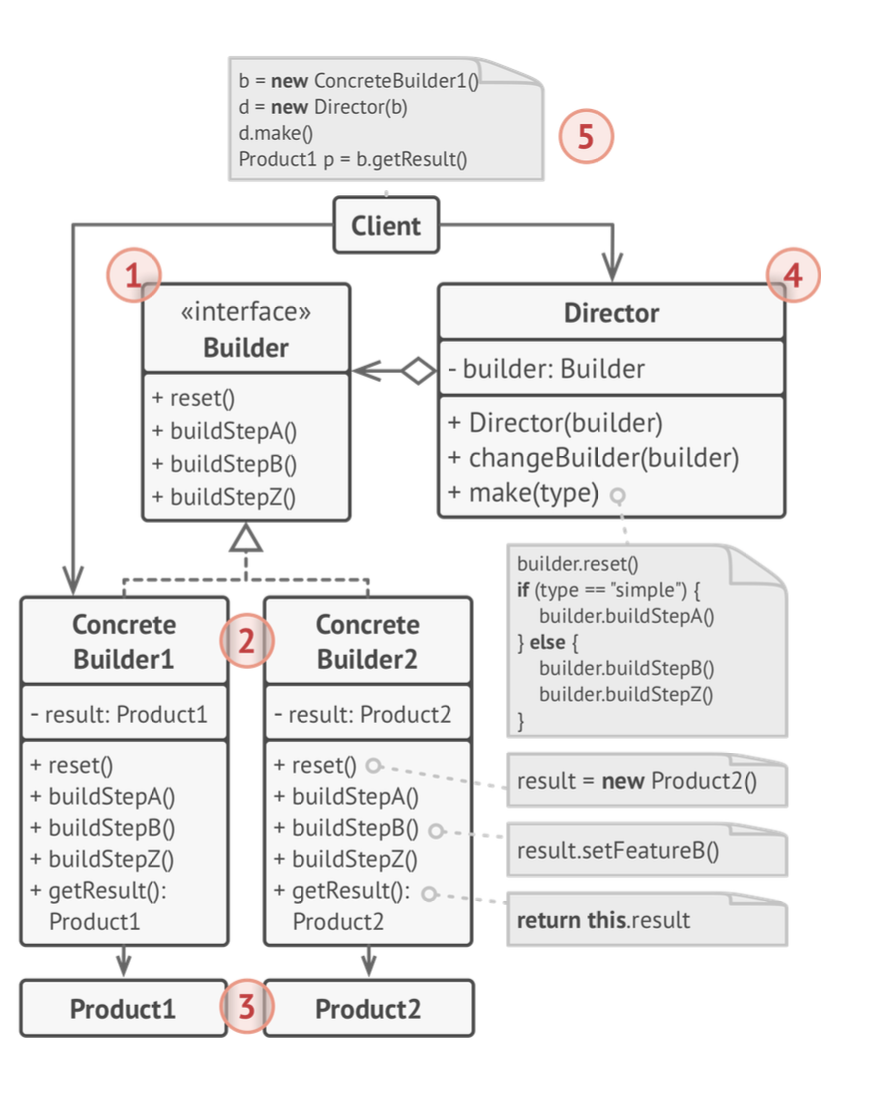
\includegraphics[width=\columnwidth]{Builder.png} % Example image
	\caption{Builder Structure}
	\label{Builder Structure}
\end{figure}

Diagram of structure Figure:\ref{Builder Structure} on Page:\pageref{Builder Structure}.

\subsection{Prototype}

Copy existing objects without dependancy.\\

Create a cloning interface common to objects that are to be duplicated. The implementation of the interface
will have a method to clone all fields of that object.\\

Good for when many objects are storing state, easy way to get an object with a basic configuration.
May not have access to all fields of an object to clone.\\

\begin{figure}[h] % [h] forces the figure to be output where it is defined in the code (it suppresses floating)
	\centering
	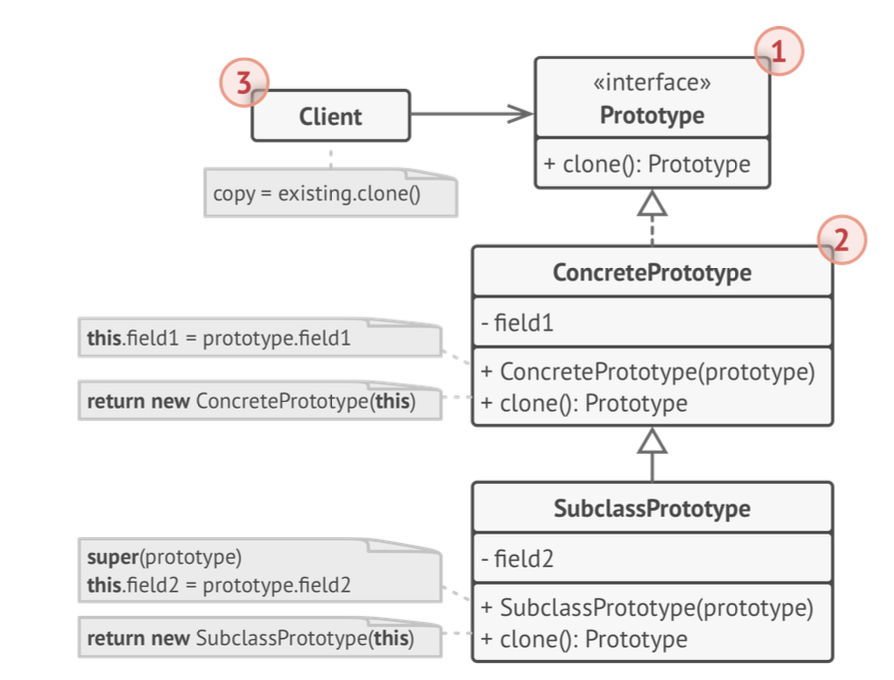
\includegraphics[width=\columnwidth]{Prototype.png} % Example image
	\caption{Prototype Structure}
	\label{Prototype Structure}
\end{figure}

Diagram of structure Figure:\ref{Prototype Structure} on Page:\pageref{Prototype Structure}.

\subsection{Singleton}

Uses only one instance that is globally available. Help protect from threading issues a shared resource.\\

Make constructor of object private, used via method in module that creates ans stores object. When called
will return created object.\\

\begin{figure}[h] % [h] forces the figure to be output where it is defined in the code (it suppresses floating)
	\centering
	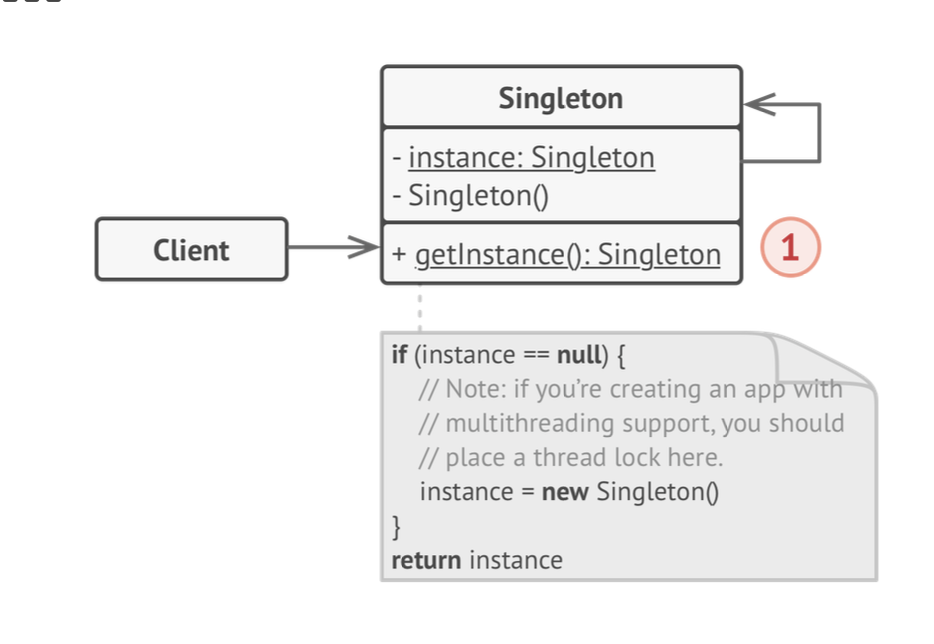
\includegraphics[width=\columnwidth]{Singleton.png} % Example image
	\caption{Singleton Structure}
	\label{Singleton Structure}
\end{figure}

Diagram of structure Figure:\ref{Singleton Structure} on Page:\pageref{Singleton Structure}.

\section{Structural Patterns}

\subsection{Adapter}

Communication between incompatible interfaces.\\

Using an interface when implemented will convert the type of one object to another by wrapping it (referencing it).
Access to the methods of the object are then via the interface. Allowing a plugin model for adapters.\\

\begin{figure}[h] % [h] forces the figure to be output where it is defined in the code (it suppresses floating)
	\centering
	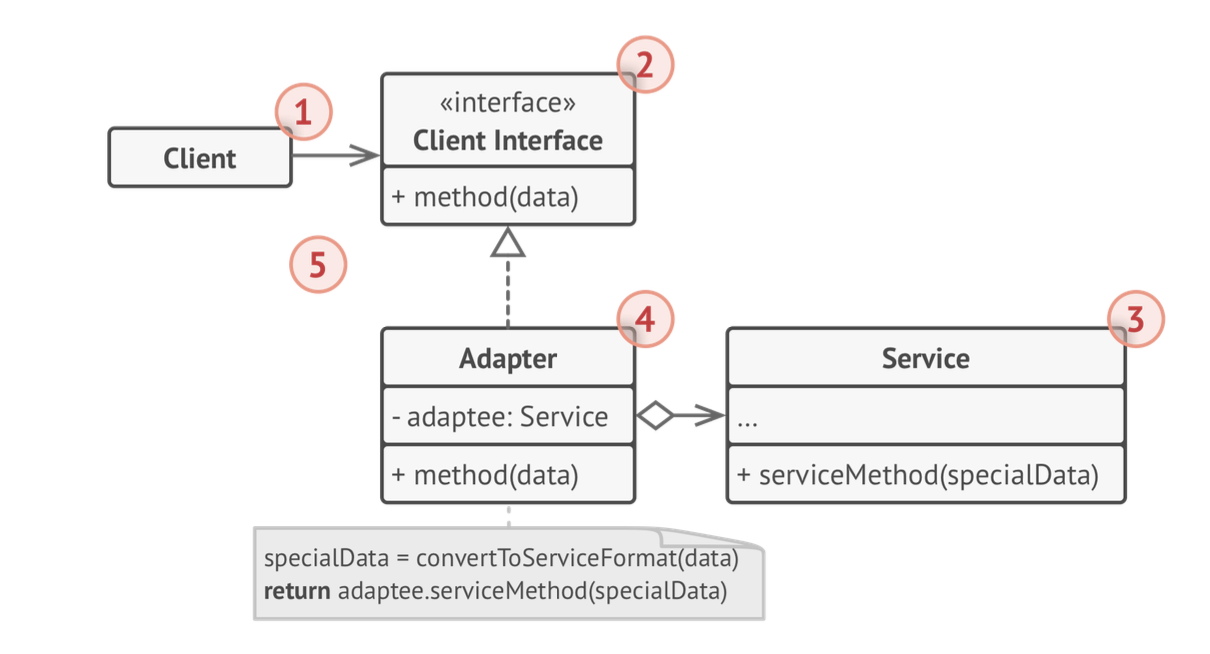
\includegraphics[width=\columnwidth]{Adapters.png} % Example image
	\caption{Adapters Structure}
	\label{Adapters Structure}
\end{figure}

Diagram of structure Figure:\ref{Adapters Structure} on Page:\pageref{Adapters Structure}.

\subsection{Bridge}

Separate modules that are the implementations and abstract.\\

Modules write high level methods that uses an interface for details to create a plugin nature. The 
abstract methods use the implementations via the interface.\\

\begin{figure}[h] % [h] forces the figure to be output where it is defined in the code (it suppresses floating)
	\centering
	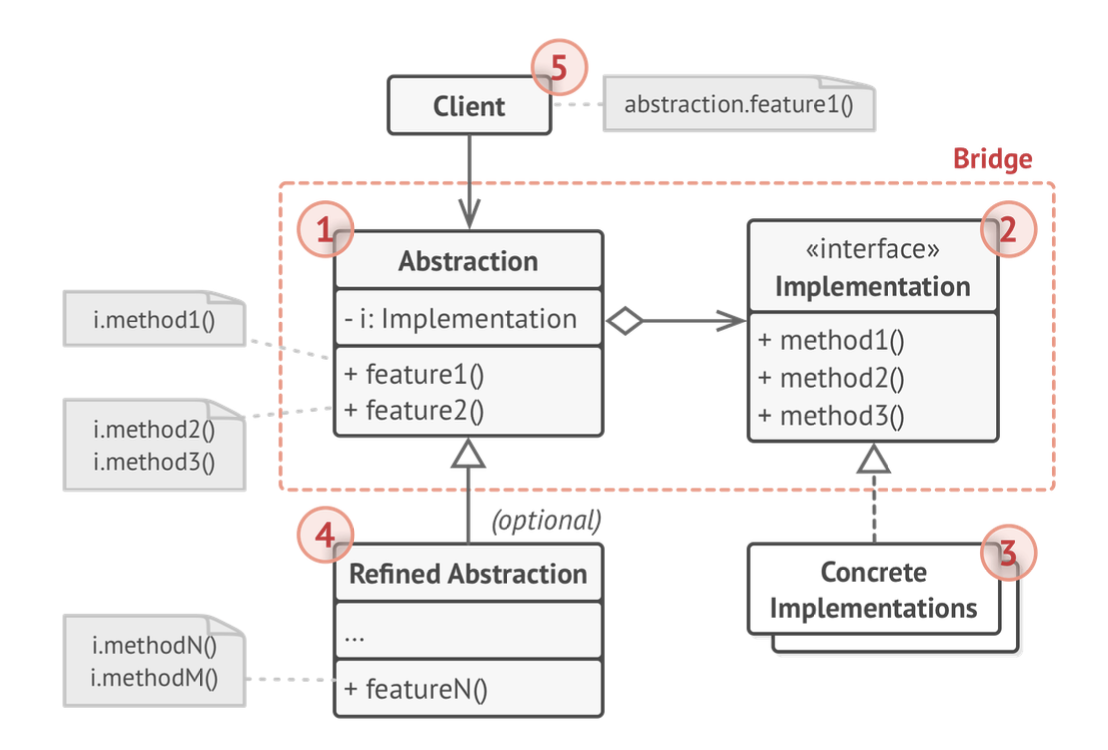
\includegraphics[width=\columnwidth]{Bridge.png} % Example image
	\caption{Bridge Structure}
	\label{Bridge Structure}
\end{figure}

Diagram of structure Figure:\ref{Bridge Structure} on Page:\pageref{Bridge Structure}.

\subsection{Composite}

Objects in tree structure.\\

Deal with all bottom leaves and higher leaves with children in the same, allowing recursion to navigate through
the tree and provide a result. A common interface is used to access each leaf, allowing an implementation be for a 
bottom leaf or an adult leaf, for the client its does not matter.\\

\begin{figure}[h] % [h] forces the figure to be output where it is defined in the code (it suppresses floating)
	\centering
	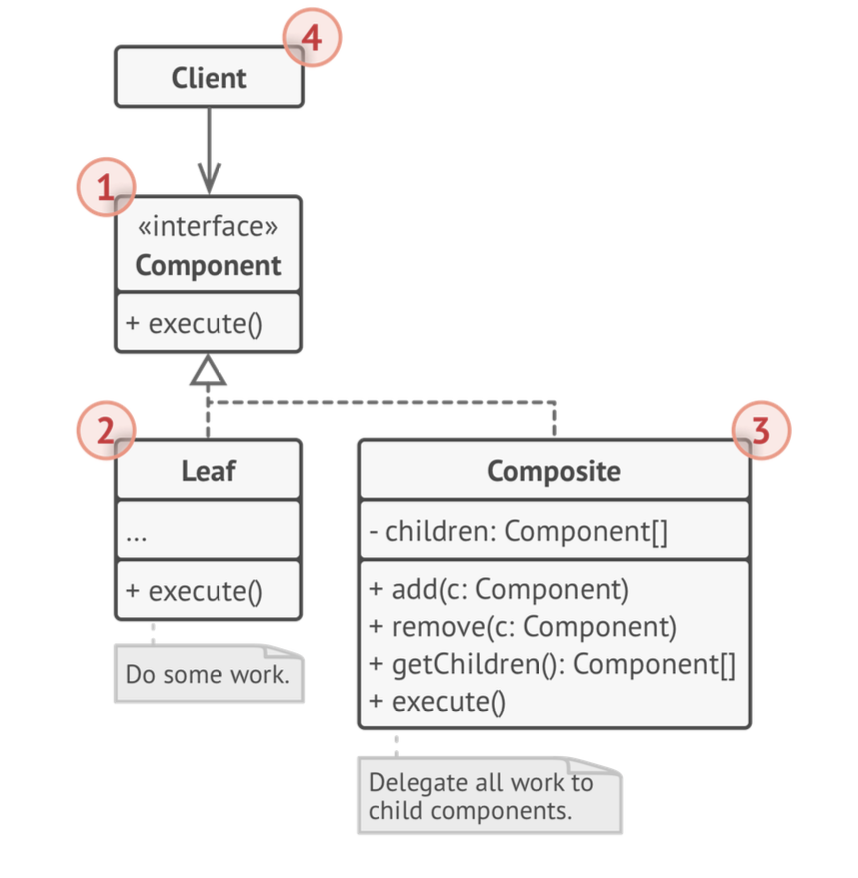
\includegraphics[width=\columnwidth]{Composite.png} % Example image
	\caption{Composite Structure}
	\label{Composite Structure}
\end{figure}

Diagram of structure Figure:\ref{Composite Structure} on Page:\pageref{Composite Structure}.

\subsection{Decorator}

Add new behaviours to objects via wrappers.\\

With a common interface between current object and the wrapper/decorator, a
base decorator is created which is extended and has access to the base object. Allowing use of either
base object or decorator without the client being aware.\\

\begin{figure}[h] % [h] forces the figure to be output where it is defined in the code (it suppresses floating)
	\centering
	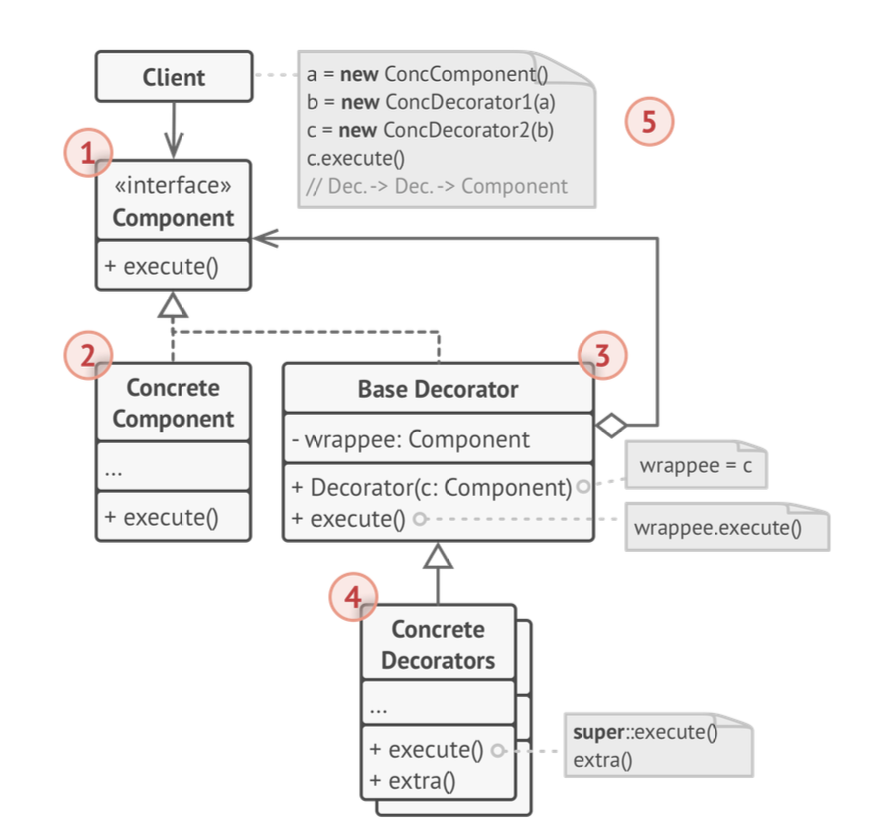
\includegraphics[width=\columnwidth]{Decorator.png} % Example image
	\caption{Decorator Structure}
	\label{Decorator Structure}
\end{figure}

Diagram of structure Figure:\ref{Decorator Structure} on Page:\pageref{Decorator Structure}.

\subsection{Facade}

Simple interface to complex objects.\\

Use an intermediary module handling all calls to the subsystem, so the client doesn't call it directly.\\

\begin{figure}[h] % [h] forces the figure to be output where it is defined in the code (it suppresses floating)
	\centering
	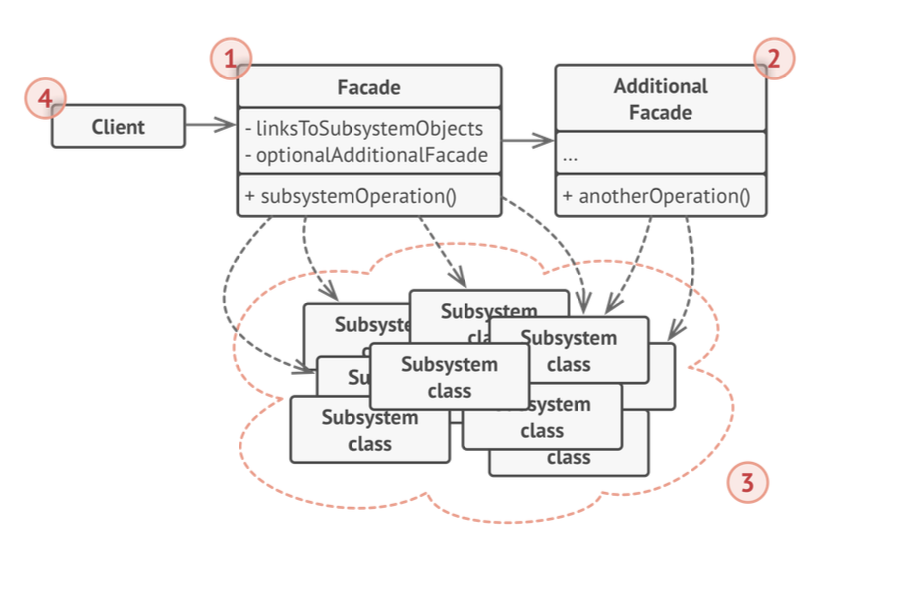
\includegraphics[width=\columnwidth]{Facade.png} % Example image
	\caption{Facade Structure}
	\label{Facade Structure}
\end{figure}

Diagram of structure Figure:\ref{Facade Structure} on Page:\pageref{Facade Structure}.

\subsection{Flyweight}

Save RAM by sharing objects.\\

Create objects "flyweights" that hold all intrinsic (not changing/identical across objects) data of objects,
which is referenced to by objects that hold the extrinsic data. The flyweights are immutable, another
module can be used to manage pools of flyweights.\\

\begin{figure}[h] % [h] forces the figure to be output where it is defined in the code (it suppresses floating)
	\centering
	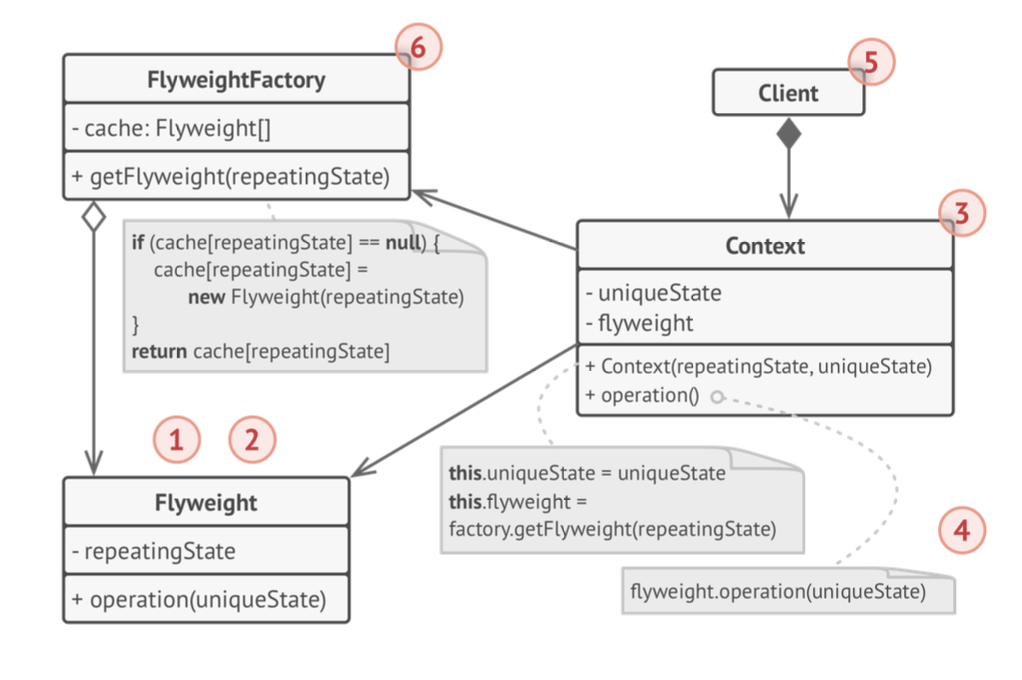
\includegraphics[width=\columnwidth]{Flyweights.png} % Example image
	\caption{Flyweights Structure}
	\label{Flyweights Structure}
\end{figure}

Diagram of structure Figure:\ref{Flyweights Structure} on Page:\pageref{Flyweights Structure}.

\subsection{Proxy}

Substitute or placeholder for object, controls access to objects so can perform methods before/after.\\

Using an interface for both the base object and proxy, with proxy linking to the service.\\

\begin{figure}[h] % [h] forces the figure to be output where it is defined in the code (it suppresses floating)
	\centering
	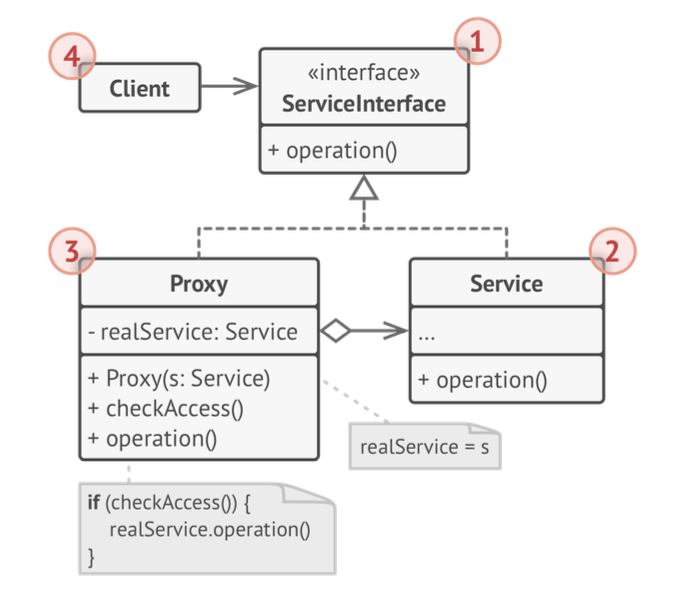
\includegraphics[width=\columnwidth]{Proxy.png} % Example image
	\caption{Proxy Structure}
	\label{Proxy Structure}
\end{figure}

Diagram of structure Figure:\ref{Proxy Structure} on Page:\pageref{Proxy Structure}.

\section{Behavioural}

\subsection{Chain of responsibility}

Pass request along chain of handlers, each handler deciding if to use it then passes it on.\\

A handler is a single module with a single method (execute) and a ref to the next handler in chain
. All handler implement the same interface, this allows the chain to be dynamically created at
run time.\\

The handler will make a decision on if the data should be passed on or if the chain can stop,
therefore only executing the number of steps required. For a cleaner setup can have a base handler
which is extended by all handlers.\\

\begin{figure}[h] % [h] forces the figure to be output where it is defined in the code (it suppresses floating)
	\centering
	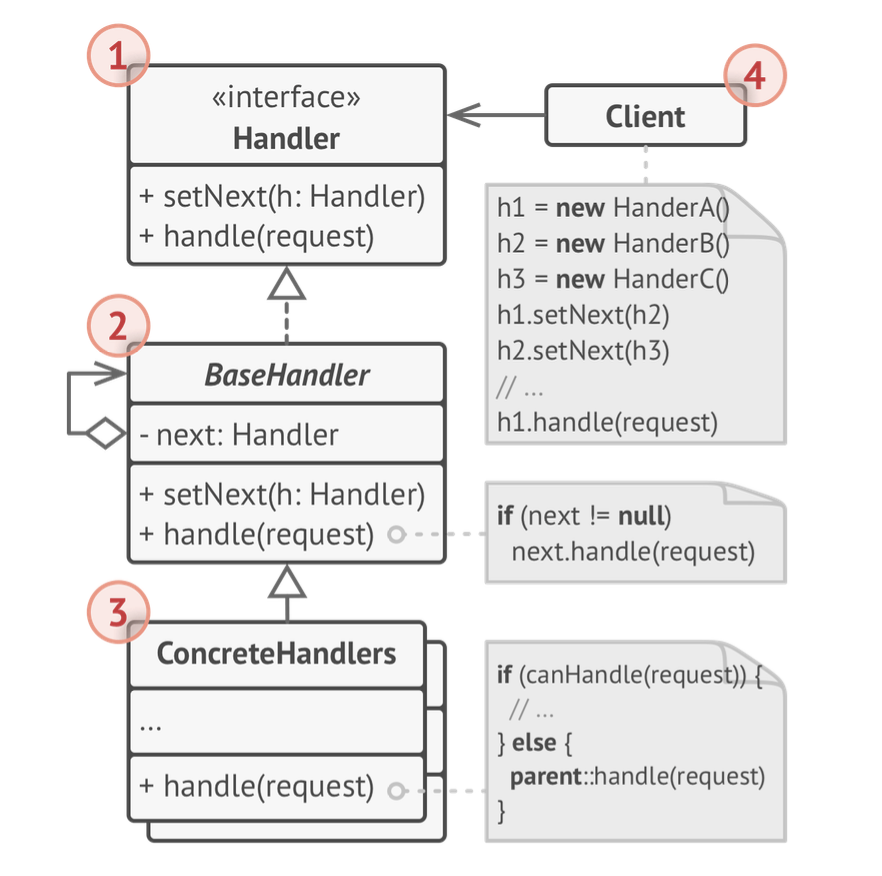
\includegraphics[width=\columnwidth]{Chain.png} % Example image
	\caption{Chain of Responsibility Structure}
	\label{Chain of Responsibility Structure}
\end{figure}

Diagram of structure Figure:\ref{Chain of Responsibility Structure} on Page:\pageref{Chain of Responsibility Structure}.

\subsection{Command}

Turn a request into an object for easier handling; can parametrise, delay or queue requests.\\

Using a 'command' module implementing an interface between procedure and low level details 
with a single execute method. Allowing the command of a interface to become a plugin. The interface
will simply alert the command, the command will then gather the data needed on its own to further decouple them.\\

If an invoker module is used to setup the required command modules and execute them when receiving a signal from the
interface can stack commands and reuse the objects.\\

\begin{figure}[h] % [h] forces the figure to be output where it is defined in the code (it suppresses floating)
	\centering
	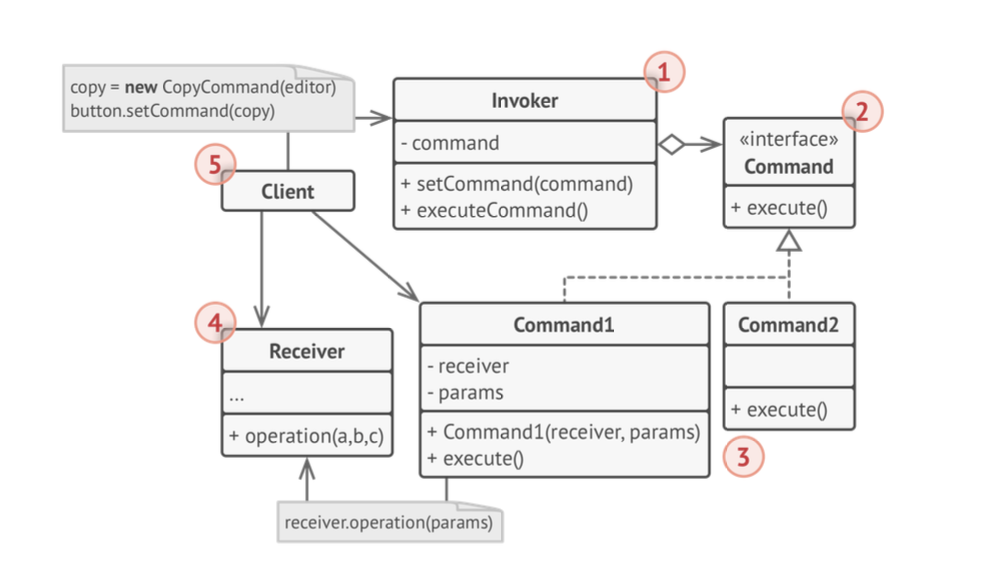
\includegraphics[width=\columnwidth]{Command.png} % Example image
	\caption{Command Structure}
	\label{Command Structure}
\end{figure}

Diagram of structure Figure:\ref{Command Structure} on Page:\pageref{Command Structure}.

\subsection{Iterator}

Traverse elements without exposing its details.\\

Storage patterns may require different traversal methods, this can be separated into modules that implement an interface.
To give the traversal a plugin nature. Can use a interable collection interface so grouping of storage method and iterators is 
easy.\\

\begin{figure}[h] % [h] forces the figure to be output where it is defined in the code (it suppresses floating)
	\centering
	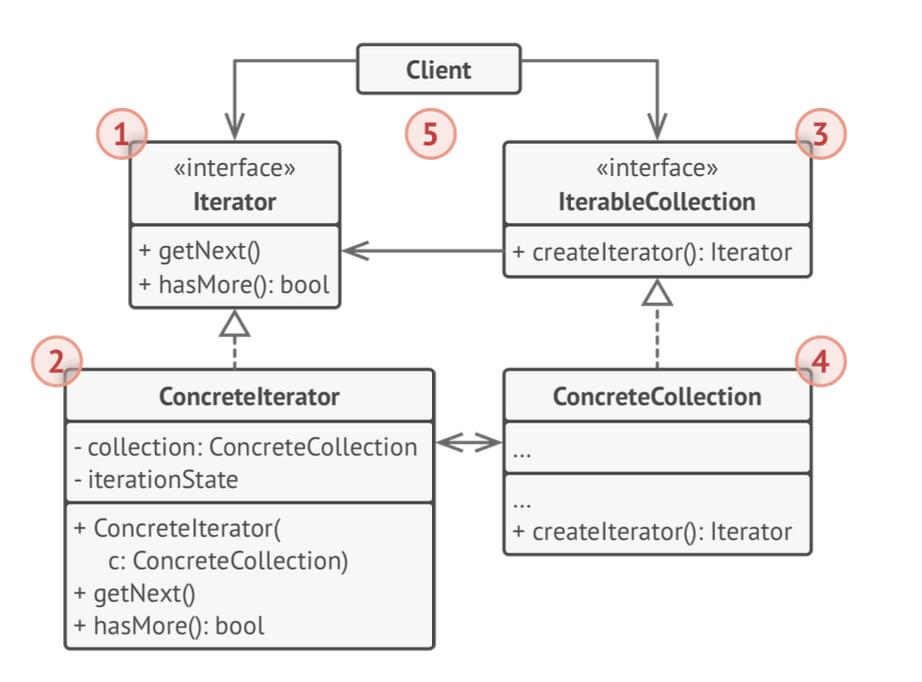
\includegraphics[width=\columnwidth]{Iterator.png} % Example image
	\caption{Iterator Structure}
	\label{Iterator Structure}
\end{figure}

Diagram of structure Figure:\ref{Iterator Structure} on Page:\pageref{Iterator Structure}.

\subsection{Mediator}

Reduce dependencies between objects and by controlling communication.\\

Components that are independent should not directly communicate, better to go via a mediator that redirects calls
based on needs. So the components depend on the mediator and not on each other. Can use an interface for using
multiple mediators, so that each component use the interface further decoupling further the interfaces.\\

Should be careful of the size of the mediator.\\

\begin{figure}[h] % [h] forces the figure to be output where it is defined in the code (it suppresses floating)
	\centering
	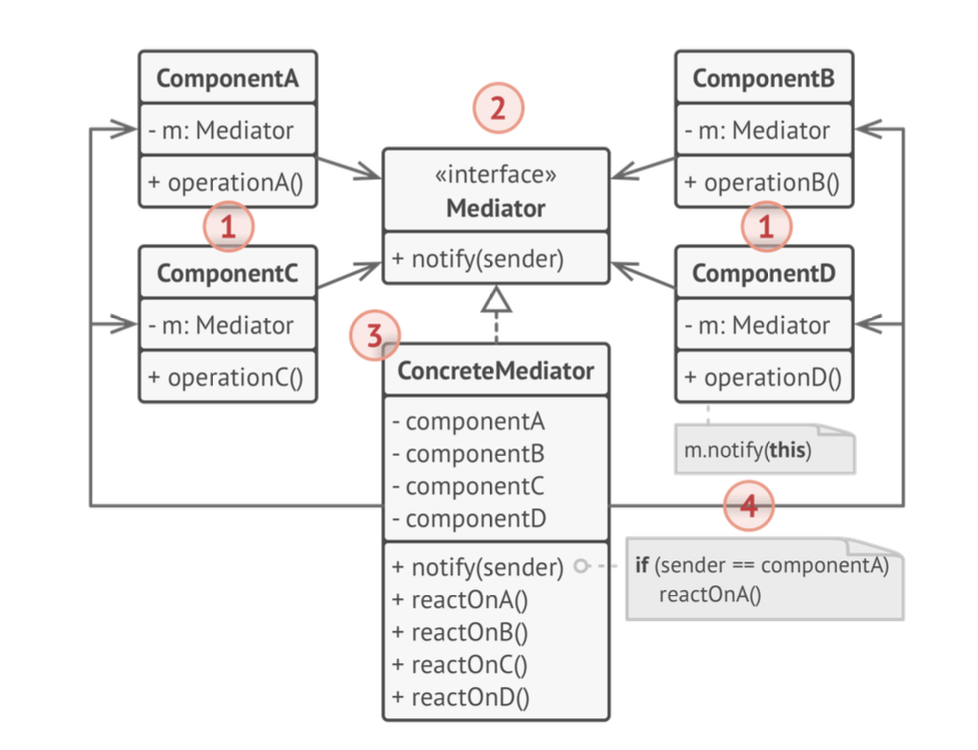
\includegraphics[width=\columnwidth]{Mediator.png} % Example image
	\caption{Mediator Structure}
	\label{Mediator Structure}
\end{figure}

Diagram of structure Figure:\ref{Mediator Structure} on Page:\pageref{Mediator Structure}.

\subsection{Memento}

Save and restore previous state of an object.\\

Best method is to allow the object to create a copy of its own state to not void the encapsulation. The copy of the state
is a special object called memento. A separate Caretaker can then store this object.\\

The memento can be created by the original object via an interface, allowing multiple memento to be used polymorphically.\\

\begin{figure}[h] % [h] forces the figure to be output where it is defined in the code (it suppresses floating)
	\centering
	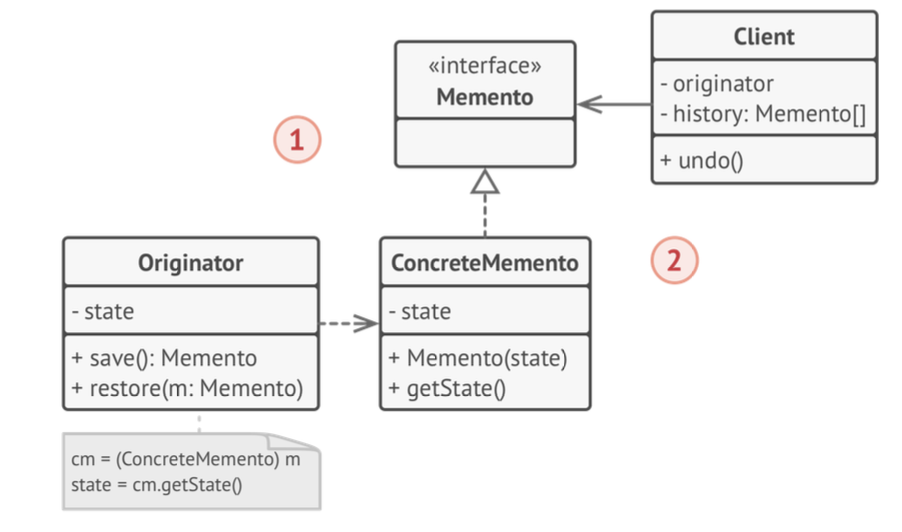
\includegraphics[width=\columnwidth]{Memento.png} % Example image
	\caption{Memento Structure}
	\label{Memento Structure}
\end{figure}

Diagram of structure Figure:\ref{Memento Structure} on Page:\pageref{Memento Structure}.

\subsection{Observer}

Notify events occurring of an observed object.\\

Via an interface a publisher module will communicate to subscribers. The publisher will hold a list of all subscribers,
with methods to add or remove a sub. Can also have a interface for the publisher.\\

\begin{figure}[h] % [h] forces the figure to be output where it is defined in the code (it suppresses floating)
	\centering
	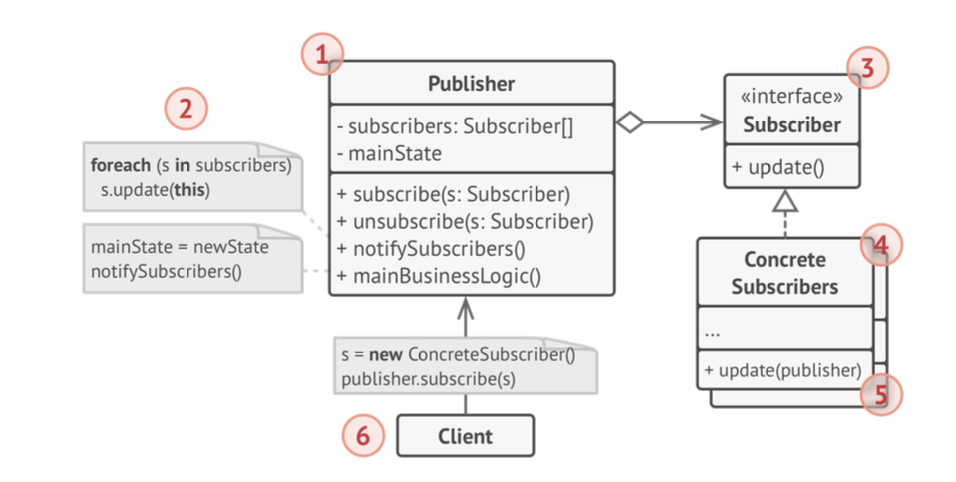
\includegraphics[width=\columnwidth]{Publisher.png} % Example image
	\caption{Publisher Structure}
	\label{Publisher Structure}
\end{figure}

Diagram of structure Figure:\ref{Publisher Structure} on Page:\pageref{Publisher Structure}.

\subsection{State}

Change behaviour based on state.\\

Finite state machine are normally based on conditionals, but this lacks evolvability. Each state has its own module,
with the original object holding a ref to its current state. And a method to change states with the state
implementations holding the state specific behaviour which is accessed via the interface. \\

The states are implemented via an interface, easy adding of states.\\

\begin{figure}[h] % [h] forces the figure to be output where it is defined in the code (it suppresses floating)
	\centering
	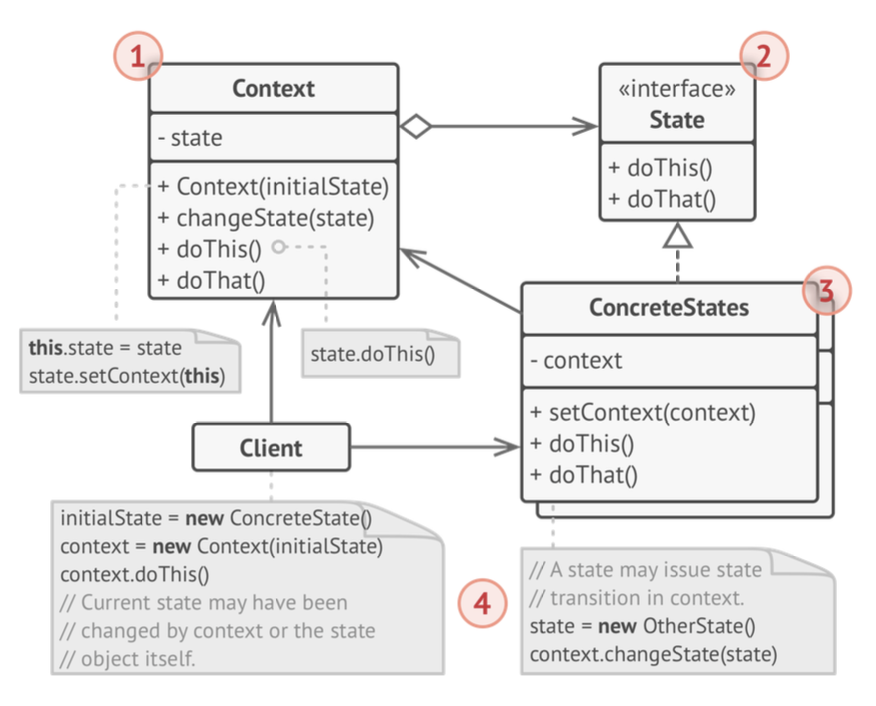
\includegraphics[width=\columnwidth]{State.png} % Example image
	\caption{State Structure}
	\label{State Structure}
\end{figure}

Diagram of structure Figure:\ref{State Structure} on Page:\pageref{State Structure}.

\subsection{Strategy}

Define a family of algorithms with each object interchangeable.\\

Split modules an implement via an interface an algorithm that does something specific in many ways. Use a context 
module to keep track of the strategies and allow use via interface. The client will then decide which strategy to use.
Context module used for cleanliness.\\

\begin{figure}[h] % [h] forces the figure to be output where it is defined in the code (it suppresses floating)
	\centering
	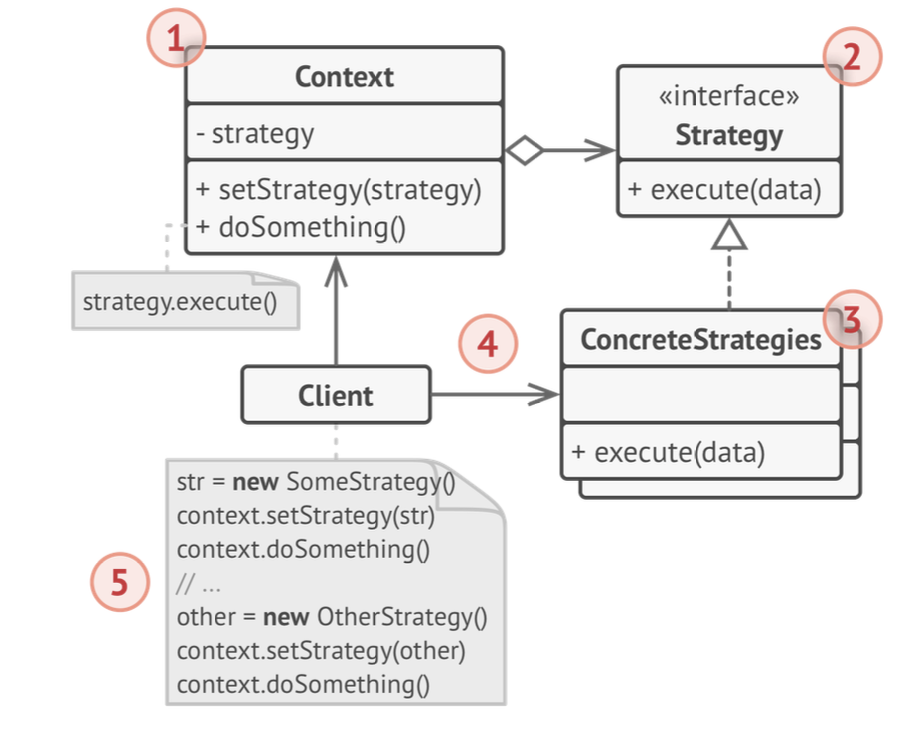
\includegraphics[width=\columnwidth]{Strategy.png} % Example image
	\caption{Strategy Structure}
	\label{Strategy Structure}
\end{figure}

Can use a set of anonymous functions instead of this interface pattern; functions without an identifier. This 
allows you to set the different functions in the context module at compile time to be used and easily add.\\

Diagram of structure Figure:\ref{Strategy Structure} on Page:\pageref{Strategy Structure}.

\subsection{Template Method}

Define structure of procedure and then adjust via subclasses.\\

The high level module will have abstract methods which have to be implemented by extensions and optional methods.\\

\begin{figure}[h] % [h] forces the figure to be output where it is defined in the code (it suppresses floating)
	\centering
	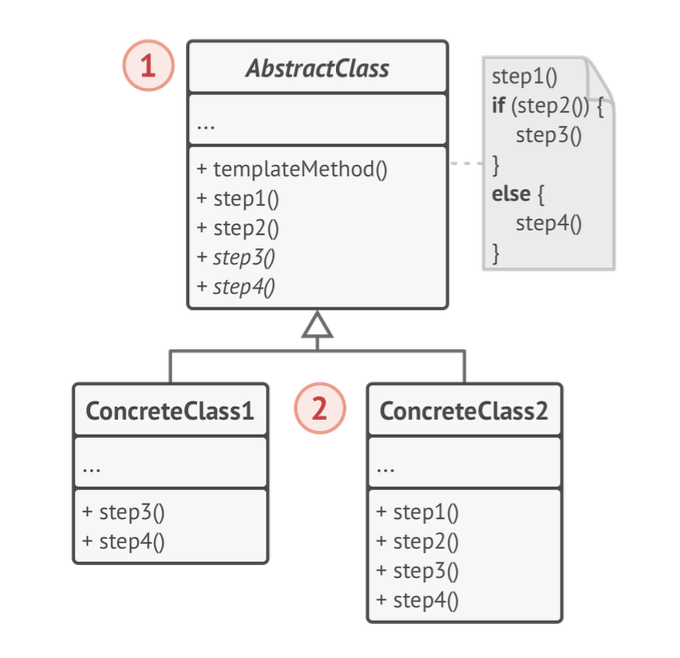
\includegraphics[width=\columnwidth]{Template.png} % Example image
	\caption{Template Method Structure}
	\label{Template Method Structure}
\end{figure}

Diagram of structure Figure:\ref{Template Method Structure} on Page:\pageref{Template Method Structure}.

\subsection{Visitor}

Separate algorithms from objects on which they operate.\\

Create a separate module for the algorithms via an interface and choose which method is require for the current object via double dispatch.
Double dispatch is when the object has a method that will use the correct method in the algorithm module accessed via
the interface.\\

Diagram of structure Figure:\ref{Visitor Structure} on Page:\pageref{Visitor Structure}.

\begin{figure}[h] % [h] forces the figure to be output where it is defined in the code (it suppresses floating)
	\centering
	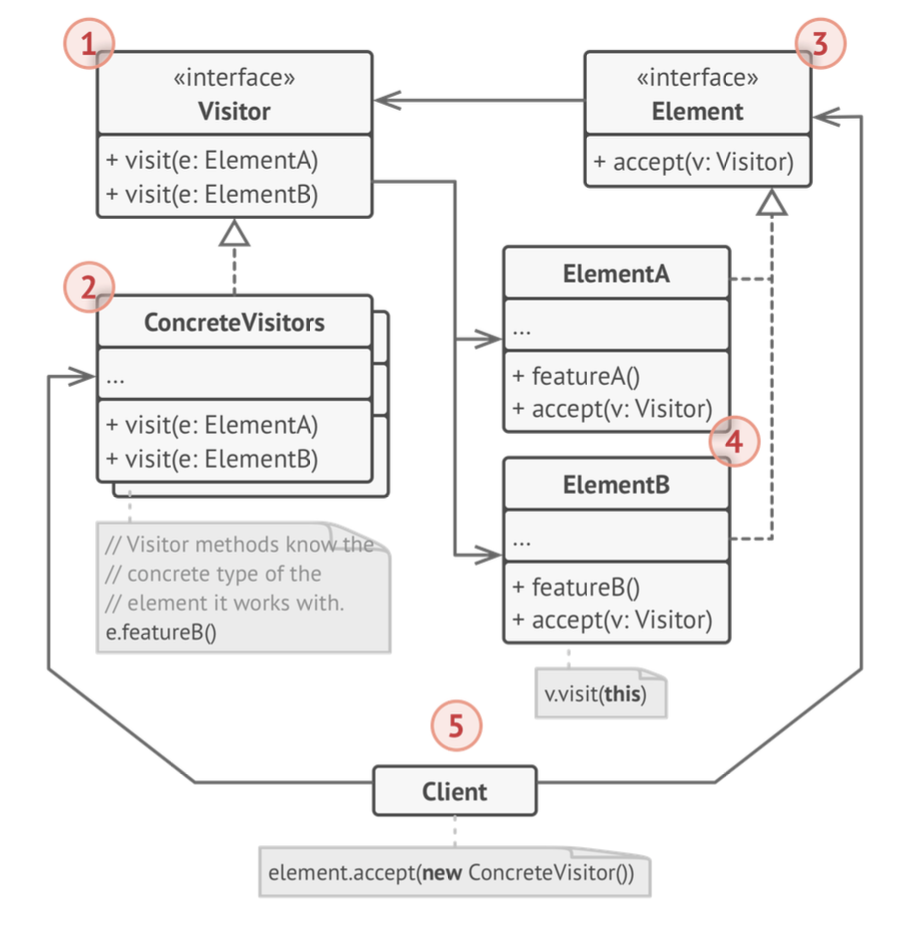
\includegraphics[width=\columnwidth]{Visitor.png} % Example image
	\caption{Visitor Structure}
	\label{Visitor Structure}
\end{figure}


%----------------------------------------------------------------------------------------
%	FIGURE EXAMPLE
%----------------------------------------------------------------------------------------

% \begin{figure}[h] % [h] forces the figure to be output where it is defined in the code (it suppresses floating)
% 	\centering
% 	\includegraphics[width=0.5\columnwidth]{IMAGE_NAME.jpg} % Example image
% 	\caption{European swallow.}
%	\label{}
% \end{figure}

%----------------------------------------------------------------------------------------
% MATH EXAMPLES
%----------------------------------------------------------------------------------------

% \begin{align} 
% 	\label{eq:bayes}
% 	\begin{split}
% 		P(A|B) = \frac{P(B|A)P(A)}{P(B)}
% 	\end{split}					
% \end{align}

%----------------------------------------------------------------------------------------
%	LIST EXAMPLES
%----------------------------------------------------------------------------------------

% \begin{itemize}
% 	\item First item in a list 
% 		\begin{itemize}
% 		\item First item in a list 
% 			\begin{itemize}
% 			\item First item in a list 
% 			\item Second item in a list 
% 			\end{itemize}
% 		\item Second item in a list 
% 		\end{itemize}
% 	\item Second item in a list 
% \end{itemize}

%------------------------------------------------

% \subsection{Numbered List}

% \begin{enumerate}
% 	\item First item in a list 
% 	\item Second item in a list 
% 	\item Third item in a list
% \end{enumerate}

%----------------------------------------------------------------------------------------
%	TABLE EXAMPLE
%----------------------------------------------------------------------------------------

% \section{Interpreting a Table}

% \begin{table}[h] % [h] forces the table to be output where it is defined in the code (it suppresses floating)
% 	\centering % Centre the table
% 	\begin{tabular}{l l l}
% 		\toprule
% 		\textit{Per 50g} & \textbf{Pork} & \textbf{Soy} \\
% 		\midrule
% 		Energy & 760kJ & 538kJ\\
% 		Protein & 7.0g & 9.3g\\
% 		\bottomrule
% 	\end{tabular}
% 	\caption{Sausage nutrition.}
% \end{table}

%----------------------------------------------------------------------------------------
%	CODE LISTING EXAMPLE
%----------------------------------------------------------------------------------------

% \begin{lstlisting}[
% 	caption= Macro definition, % Caption above the listing
% 	language=python, % Use Julia functions/syntax highlighting
% 	frame=single, % Frame around the code listing
% 	showstringspaces=false, % Don't put marks in string spaces
% 	numbers=left, % Line numbers on left
% 	numberstyle=\large, % Line numbers styling
% 	]

% 	CODE

% \end{lstlisting}

%----------------------------------------------------------------------------------------
%	CODE LISTING FILE EXAMPLE
%----------------------------------------------------------------------------------------

% \lstinputlisting[
% 	caption=Luftballons Perl Script., % Caption above the listing
% 	label=lst:luftballons, % Label for referencing this listing
% 	language=Perl, % Use Perl functions/syntax highlighting
% 	frame=single, % Frame around the code listing
% 	showstringspaces=false, % Don't put marks in string spaces
% 	numbers=left, % Line numbers on left
% 	numberstyle=\tiny, % Line numbers styling
% 	]{luftballons.pl}

%----------------------------------------------------------------------------------------
%	BIB EXAMPLE
%----------------------------------------------------------------------------------------

% Using \texttt{biblatex} you can display a bibliography divided into sections, depending on citation type. 
% Let's cite! Einstein's journal paper \cite{einstein} and Dirac's book \cite{dirac} are physics-related items. 
% Next, \textit{The \LaTeX\ Companion} book \cite{latexcompanion}, Donald Knuth's website \cite{knuthwebsite}, \textit{The Comprehensive Tex Archive Network} (CTAN) \cite{ctan} are \LaTeX-related items; but the others, Donald Knuth's items, \cite{knuth-fa,knuth-acp} are dedicated to programming. 

% \medskip

% \printbibliography[
% heading=bibintoc,
% title={Whole bibliography}
% ] %Prints the entire bibliography with the title "Whole bibliography"

% %Filters bibliography
% \printbibliography[heading=subbibintoc,type=article,title={Articles only}]
% \printbibliography[type=book,title={Books only}]

% \printbibliography[keyword={physics},title={Physics-related only}]
% \printbibliography[keyword={latex},title={\LaTeX-related only}]

\end{document}